\documentclass[11pt,class=report,crop=false]{standalone}
\usepackage[screen]{../python}

\begin{document}


%====================================================================
\chapitre{Fonctions}
%====================================================================

\objectifs{\'Ecrire une fonction, c'est la façon la plus simple de regrouper du code pour une tâche bien particulière, dans le but de l'exécuter une ou plusieurs fois par la suite.}

\begin{cours}[Fonction (début)]

\index{fonction}

Une fonction en informatique est une portion réalisant un tâche bien précise et qui pourra être utilisée une ou plusieurs fois dans la suite du programme. 
Pour définir une fonction avec \Python{}, c'est très simple. 
Voici deux exemples :
\begin{center}
\begin{minipage}{0.4\textwidth}
\begin{lstlisting}
def dit_bonjour():
    print("Bonjour le monde !")
    return
\end{lstlisting}
\end{minipage}\qquad\qquad
\begin{minipage}{0.4\textwidth}
\begin{lstlisting}
def affiche_carres():
    for i in range(20):
        print(i**2)
    return
\end{lstlisting}
\end{minipage}
\end{center}

\index{def@\ci{def}}

Les instructions sont regroupées dans un bloc indenté. Le mot \ci{return}\index{return@\ci{return}} (optionnel) indique la fin de la fonction. Ces instructions ne sont exécutées que si j'appelle la fonction. Par exemple, chaque fois que j'exécute la commande \ci{dit_bonjour()}, \Python{} affiche la phrase \og{}Bonjour le monde !\fg{}. Chaque fois que j'exécute la commande \ci{affiche_carres()}, \Python{} affiche $0,1,4,9,16,\ldots$, c'est-à-dire les nombres $i^2$ pour $i=0,\ldots,19$.

\mybox{
\myfigure{0.7}{
  \tikzinput{fig-fonctions-cours-1}
} }


\end{cours}



\begin{cours}[Fonction (suite)]

Les fonctions informatiques acquièrent tout leur potentiel avec :
\begin{itemize}
  \item une \defi{entrée}, qui regroupe des variables qui servent de \defi{paramètres}\index{parametre@paramètre}\index{fonction!parametre@paramètre},
  \item une \defi{sortie}, qui est un résultat renvoyé par la fonction (et qui souvent dépendra des paramètres d'entrée).
\end{itemize}

Voici deux exemples :
\begin{center}
\begin{lstlisting}
def affiche_mois(numero):
    if numero == 1:
        print("Nous sommes en janvier.")
    if numero == 2:
        print("Nous sommes en février.")
    if numero == 3:
        print("Nous sommes en mars.")
    # etc.
    return
\end{lstlisting}
\end{center}
Lorsqu'elle est appelée cette fonction affiche le nom du mois en fonction du nombre fourni en entrée. Par exemple \ci{affiche_mois(3)} va afficher \ci{"Nous sommes en mars."}.

\begin{center}
\begin{lstlisting}
def calcule_cube(a):
    cube = a * a * a    # ou bien a**3
    return cube
\end{lstlisting}

\end{center}

Cette fonction calcule le cube d'un nombre, par exemple \ci{calcule_cube(2)} n'affiche rien mais renvoie la valeur \ci{8}. Cette valeur peut être utilisée ailleurs dans le programme.
Par exemple, que font les instructions suivantes ?
\begin{center}
\begin{lstlisting}
x = 3
y = 4
z = calcule_cube(x) + calcule_cube(y)
print(z)
\end{lstlisting}
\end{center}
En terme mathématiques, on pose $x=3$, $y=4$, puis on calcule le cube de $x$, le cube de $y$ et on les additionne :
$$z = x^3 + y^3 = 3^3 + 4^3 = 27 + 64 = 91$$
Ainsi le programme affiche \ci{91}.
\mybox{
\myfigure{0.7}{
  \tikzinput{fig-fonctions-cours-2}
} }

Les avantages de la programmation utilisant des fonctions sont les suivants :
\begin{itemize}
  \item on écrit le code d'une fonction une seule fois, mais on peut appeler la fonction plusieurs fois ;
  \item en divisant notre programme en petits blocs ayant chacun leur utilité propre, le programme est plus facile à écrire, à lire, à corriger et à modifier ;
  \item on peut utiliser une fonction (écrite par quelqu'un d'autre, comme par exemple la fonction \ci{sqrt()}) sans connaître tous les détails internes de sa programmation.
\end{itemize} 

\end{cours}


%%%%%%%%%%%%%%%%%%%%%%%%%%%%%%%%%%%%%%%%%%%%%%%%%%%%%%%%%%%%%%%%
% Activité 1
%%%%%%%%%%%%%%%%%%%%%%%%%%%%%%%%%%%%%%%%%%%%%%%%%%%%%%%%%%%%%%%%

\begin{activite}[Premières fonctions]
\objectifs{Objectifs : écrire des fonctions très simples.}

\begin{enumerate}
  \item \textbf{Fonction sans paramètre ni sortie.}
  \begin{enumerate}
    \item Programme une fonction appelée \ci{affiche_table_de_7()} qui affiche la table de multiplication par $7$ : $1 \times 7 = 7$, $2\times 7 = 14$\ldots
    
    \item Programme une fonction appelée \ci{affiche_bonjour()} qui demande à l'utilisateur son prénom et affiche ensuite \og{}Bonjour\fg{} suivi du prénom de l'utilisateur.
    
    \emph{Indication.} Utilise \ci{input()}.
  \end{enumerate}

  \item \textbf{Fonction avec un paramètre et sans sortie.}
  \begin{enumerate}
    \item Programme une fonction appelée \ci{affiche_une_table(n)} qui dépend d'un paramètre \ci{n} et qui affiche la table de multiplication par l'entier $n$.
    Par exemple, la commande \ci{affiche_une_table(5)} doit afficher : $1 \times 5 = 5$, $2\times 5 = 10$\ldots
    
    \item Programme une fonction appelée \ci{affiche_salutation(formule)} qui dépend d'un paramètre \ci{formule}. Cette fonction demande le prénom de l'utilisateur et affiche une formule de salutation suivi du prénom. Par exemple \ci{affiche_salutation("Coucou")} afficherait \og{}Coucou\fg{} suivi du prénom donné par l'utilisateur.
  \end{enumerate}  
  
  \item \textbf{Fonction sans paramètre et avec sortie.}
  
Programme une fonction appelée \ci{demande_prenom_nom()} qui demande d'abord le prénom de l'utilisateur, puis son nom et renvoie comme résultat l'identité complète avec le nom en majuscule. Par exemple, si l’utilisateur saisi \og{}Dark\fg{} puis \og{}Vador\fg{}, la fonction renvoie la chaîne \ci{"Dark VADOR"} (la fonction n'affiche rien).

\emph{Indications.} 
\begin{itemize}
  \item Si \ci{chaine} est une chaîne de caractères, alors \ci{chaine.upper()}\index{chaine@chaîne!majuscule}\index{majuscule}\index{upper@\ci{upper}} est la chaîne transformée avec les caractères en majuscules. Exemple : si \ci{chaine = "Vador"} alors \ci{chaine.upper()} renvoie \ci{"VADOR"}.
  
  \item \index{concatenation@concaténation} On peut fusionner deux chaînes en utilisant le signe \og{}\ci{+}\fg{}. Exemple : \ci{"Dark" + "Vador"} vaut \ci{"DarkVador"}.  Autre exemple : si \ci{chaine1 = "Dark"} et \ci{chaine2 = "Vador"} alors \ci{chaine1 + " " + chaine2} vaut \ci{"Dark Vador"}.
\end{itemize}
\end{enumerate}
\end{activite}


%%%%%%%%%%%%%%%%%%%%%%%%%%%%%%%%%%%%%%%%%%%%%%%%%%%%%%%%%%%%%%%%
%%%%%%%%%%%%%%%%%%%%%%%%%%%%%%%%%%%%%%%%%%%%%%%%%%%%%%%%%%%%%%%%

\begin{cours}[Fonction (suite et fin pour l'instant)]

Une fonction peut avoir plusieurs paramètres et renvoyer plusieurs résultats.
Par exemple, voici une fonction qui calcule et renvoie la somme et le produit de deux nombres donnés en entrée.

\begin{center}
\begin{lstlisting}
def somme_produit(a,b):
    """Calcule la somme et le produit de deux nombres"""
    s = a + b
    p = a * b
    return s, p
    
som, pro = somme_produit(6,7)
\end{lstlisting}
\end{center}

La dernière ligne appelle la fonction avec les arguments $6$ (pour le paramètre \ci{a}) et $7$ (pour le paramètre \ci{b}). Cette fonction renvoie deux valeurs, la première est affectée à \ci{som} (qui vaut donc ici $13$) et la seconde à \ci{pro} (qui vaut donc $42$).

\mybox{
\myfigure{0.7}{
  \tikzinput{fig-fonctions-cours-3}
} }

Retenons donc :
\begin{itemize}
  \item Il peut y avoir plusieurs paramètres en entrée.
  
  \item Il peut y avoir plusieurs résultats en sortie.
  
  \item Très important ! Il ne faut pas confondre afficher et renvoyer une valeur.
  L'affichage (par la commande \ci{print()}) affiche juste quelque chose à l'écran. La plupart des fonctions n'affichent rien, mais renvoient une valeur (ou plusieurs). C'est beaucoup plus utile car cette valeur peut être utilisée ailleurs dans le programme.
  
  \item Dès que le programme rencontre l'instruction \ci{return}\index{return@\ci{return}}\index{fonction!return@\ci{return}}, la fonction s'arrête et renvoie le résultat. Il peut y avoir plusieurs fois l'instruction \ci{return} dans une fonction mais une seule sera exécutée. On peut aussi ne pas mettre d'instruction \ci{return} si la fonction ne renvoie rien.
  
  \item Dans les instructions d'une fonction, on peut bien sûr faire appel à d'autres fonctions !
   
  \item Il est important de bien commenter tes programmes. Pour documenter une fonction, tu peux décrire ce qu'elle fait en commençant par un \emph{docstring}\index{docstring@\emph{docstring}}\index{fonction!docstring@\emph{docstring}}, c'est-à-dire une description (en français) entourée par trois guillemets : \ci{""" Ma fonction fait ceci et cela. """} à placer juste après l'entête.

  
  \item Lorsque l'on définit une fonction, les variables qui apparaissent entre les parenthèses sont appelées les \defi{paramètres} ; par contre, lorsque l'on appelle la fonction, les valeurs entre les parenthèses sont appelées les \defi{arguments}\index{argument}\index{fonction!argument}. Il y a bien sûr une correspondance entre les deux.

  

\end{itemize}
\end{cours}


%%%%%%%%%%%%%%%%%%%%%%%%%%%%%%%%%%%%%%%%%%%%%%%%%%%%%%%%%%%%%%%%
% Activité 2
%%%%%%%%%%%%%%%%%%%%%%%%%%%%%%%%%%%%%%%%%%%%%%%%%%%%%%%%%%%%%%%%

\begin{activite}[Encore des fonctions]

\objectifs{Objectifs : construire des fonctions avec différents types d'entrée et de sortie.}

\begin{enumerate}
  \item \textbf{Trinômes.}
  
  \begin{enumerate}
    \item Écris une fonction \ci{trinome_1(x)} qui dépend d'un paramètre \ci{x} et qui renvoie la valeur du trinôme $3x^2-7x+4$. Par exemple \ci{trinome_1(7)} renvoie \ci{102}.
    
    \item Écris une fonction \ci{trinome_2(a,b,c,x)} qui dépend de quatre paramètres \ci{a}, \ci{b}, \ci{c} et \ci{x} et qui renvoie la valeur du trinôme $ax^2+bx+c$. Par exemple \ci{trinome_2(2,-1,0,6)} renvoie \ci{66}.
  \end{enumerate}   
  
  
  \item \textbf{Devises.}
  
   \begin{enumerate}
    \item Écris une fonction \ci{conversion_euros_vers_dollars(montant)} qui dépend d'un paramètre et qui pour une somme d'argent \ci{montant}, exprimée en euros, renvoie sa valeur en dollars (tu prendras par exemple $1$ euro = $1,15$ dollar).
    
    \item Écris une fonction \ci{conversion_euros(montant,devise)} qui dépend d'un paramètre \ci{montant} et d'une monnaie \ci{devise} et qui convertit la somme \ci{montant} donnée en euros, dans la devise souhaitée.
    Exemples de devises : 
    $1$ euro = $1,15$ dollar ;
    $1$ euro = $0,81$ livre ;
    $1$ euro = $130$ yens.
    Par exemple \ci{conversion_euros(100,"livre")} renvoie $81$.   
    
    
  \emph{Prends soin de donner un nom intelligible à tes fonctions ainsi qu'aux variables. N'oublie pas de documenter chaque fonction en ajoutant un petit texte explicatif entre triples guillemets au tout début de ta fonction.}
    
    
  \end{enumerate}   
  
  \item \textbf{Volumes.}
  
   Construis des fonctions qui calculent et renvoient des volumes :
  \begin{itemize}
    \item le volume d'un cube en fonction de la longueur d'un côté,
    \item le volume d'une boule en fonction de son rayon,
    \item le volume d'un cylindre en fonction du rayon de sa base et de sa hauteur,
    \item le volume d'une boîte parallélépipède rectangle en fonction de ses trois dimensions.
   \end{itemize}
   
   Pour la valeur de $\pi$, tu prendras soit la valeur approchée $3.14$, soit la valeur approchée fournie par la constante \ci{pi} du module \ci{math}.
  
  
  \item \textbf{Périmètres et aires.}
  
  \begin{enumerate}
    \item Écris une fonction dont l'usage est \ci{perimetre_aire_rectangle(a,b)} et qui renvoie en sortie le périmètre et l'aire d'un rectangle de dimensions $a$ et $b$.
   
    
    \item Même question avec \ci{perimetre_aire_disque(r)} pour le périmètre et l'aire d'un disque de rayon $r$.
    
    \item Utilise ta fonction précédente pour conjecturer à partir de quel rayon, l'aire d'un disque est plus grande que le périmètre de ce disque.
    
    \emph{Indication.} Si tu veux balayer les rayons en incrémentant la valeur de $0.1$ à chaque fois, tu peux construire une boucle ainsi :\\
    \centerline{\ci{for rayon in range(0,30):}}
    puis faire un appel à la fonction par \ci{perimetre_aire_disque(rayon/10)}.
  \end{enumerate}
\end{enumerate}
  

\end{activite}




%%%%%%%%%%%%%%%%%%%%%%%%%%%%%%%%%%%%%%%%%%%%%%%%%%%%%%%%%%%%%%%%
% Activité 3
%%%%%%%%%%%%%%%%%%%%%%%%%%%%%%%%%%%%%%%%%%%%%%%%%%%%%%%%%%%%%%%%

\begin{activite}[Tortue]
\index{tortue}

\objectifs{Objectifs : définir quelques fonctions qui dessinent des figures géométriques. Créer une fonction est similaire à créer un bloc avec \emph{Scratch}.}

\begin{center}
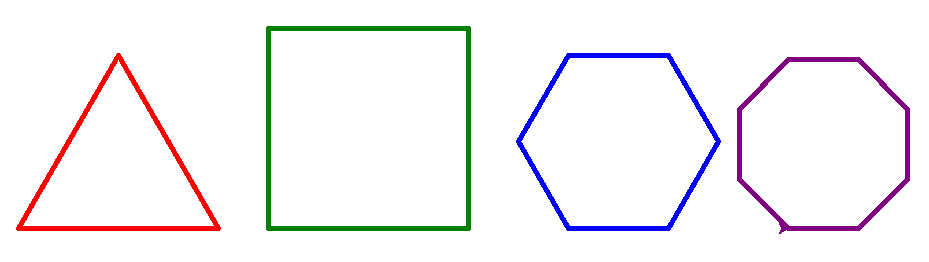
\includegraphics[scale=0.4]{ecran-fonctions-tortue}
\end{center}

\begin{enumerate}
  \item Programme une fonction \ci{triangle()} qui dessine un triangle (en rouge, chaque côté mesurant $200$).

  \item Programme une fonction \ci{carre()} qui dessine un carré (en vert, chaque côté mesurant $200$). Utilise une boucle \og{}pour\fg{} afin de ne pas avoir à réécrire les mêmes instructions plusieurs fois.  
  
  \item Programme une fonction \ci{hexagone(longueur)} qui trace un hexagone (en bleu) d'une longueur de côté donnée (l'angle pour tourner est de $60$ degrés).
  
  
  \item Programme une fonction \ci{polygone(n,longueur)} qui trace un polygone régulier à $n$ côtés et d'une longueur de côté donnée (l'angle pour tourner est alors de $360/n$ degrés). 
\end{enumerate}

\end{activite}




%%%%%%%%%%%%%%%%%%%%%%%%%%%%%%%%%%%%%%%%%%%%%%%%%%%%%%%%%%%%%%%%
% Activité 4
%%%%%%%%%%%%%%%%%%%%%%%%%%%%%%%%%%%%%%%%%%%%%%%%%%%%%%%%%%%%%%%%

\begin{activite}[Toujours des fonctions]

\objectifs{Objectifs : créer de nouvelles fonctions.}

\begin{enumerate}
  \item 
  
  \begin{enumerate}
  \item 
  Voici la réduction pour le prix d'un billet de train en fonction de l'âge du voyageur :
  \begin{itemize}
    \item réduction de $50\%$ pour les moins de $10$ ans ;
    \item réduction de $30\%$ pour les $10$ à $18$ ans ;
    \item réduction de $20\%$ pour les $60$ ans et plus.
  \end{itemize}
  
  \'Ecris une fonction \ci{reduction()} qui renvoie la réduction en fonction de l'âge et dont les propriétés sont rappelées dans le cadre ci-dessous :
\begin{fonction}[\ci{reduction()}]
  Usage : \ci{reduction(age)} \\
  Entrée : un entier correspondant à l'âge\\
  Sortie : un entier correspondant à la réduction
  
  \medskip
    
  Exemples : 
  \begin{itemize}
    \item \ci{reduction(17)} renvoie \ci{30}.
    \item \ci{reduction(23)} renvoie \ci{0}.
  \end{itemize}
  \end{fonction}  
  
  \item Déduis-en une fonction \ci{montant()} qui calcule le montant à payer en fonction du tarif normal et de l'âge du voyageur.
  
\begin{fonction}[\ci{montant()}]
  Usage : \ci{montant(tarif_normal,age)} \\
  Entrée : un nombre \ci{tarif_normal} correspondant au prix sans réduction et \ci{age} (un entier)\\
  Sortie : un nombre correspondant au montant à payer après réduction \\
  Remarque : utilise la fonction \ci{reduction()}
  \medskip
    
  Exemple : \ci{montant(100,17)} renvoie \ci{70}.
  \end{fonction} 
  
  Une famille achète des billets pour différents trajets, voici le tarif normal de chaque trajet et les âges des voyageurs : 
  \begin{itemize}
    \item tarif normal $30$ euros, enfant de $9$ ans ;
    
    \item tarif normal $20$ euros, pour chacun des jumeaux de $16$ ans ;
    
    \item tarif normal $35$ euros, pour chacun des parents de $40$ ans.
  \end{itemize}
  Quel est le montant total payé par la famille ?
 
  \end{enumerate}
  
  
  \item On souhaite programmer un petit quiz sur les tables de multiplication.
  
  \begin{enumerate}
    \item Programme une fonction \ci{calcul_est_exact()} qui décide si la réponse donnée à une multiplication est juste ou pas.
    
\begin{fonction}[\ci{calcul_est_exact()}]
  Usage : \ci{calcul_est_exact(a,b,reponse)} \\
  Entrée : trois entiers, \ci{reponse} étant la réponse proposée au calcul de $a \times b$.\\
  Sortie : \og{}vrai\fg{} ou \og{}faux\fg{}, selon que la réponse est correcte ou pas
  
  \medskip
    
  Exemples : 
  \begin{itemize}
    \item \ci{calcul_est_exact(6,7,35)} renvoie \ci{False}.
    \item \ci{calcul_est_exact(6,7,42)} renvoie \ci{True}.
  \end{itemize}
  \end{fonction}  
  
  
    \item Programme une fonction qui affiche une multiplication, demande une réponse et affiche une petite phrase de conclusion. Tout cela en français ou en anglais !
    
\begin{fonction}[\ci{test_multiplication()}]
  Usage : \ci{test_multiplication(a,b,lang)} \\
  Entrée : deux entiers, la langue choisie (parmi \ci{"francais"} ou \ci{"anglais"})\\
  Sortie : rien\\
  Remarque : utilise la fonction \ci{calcul_est_exact()}
  
  \medskip
    
  Exemple : \ci{test_multiplication(6,7,"anglais")} demande, en anglais, la réponse au calcul $6 \times 7$ et répond si c'est correct ou pas.
  \end{fonction}     
    
  \end{enumerate}
  
  
  \textbf{Bonus.} Améliore ton programme afin que l'ordinateur propose tout seul des opérations aléatoires au joueur. (Utilise la fonction \ci{randint()} du module \ci{random}.)
  
\end{enumerate}
\end{activite}




%%%%%%%%%%%%%%%%%%%%%%%%%%%%%%%%%%%%%%%%%%%%%%%%%%%%%%%%%%%%%%%%
% Activité 5
%%%%%%%%%%%%%%%%%%%%%%%%%%%%%%%%%%%%%%%%%%%%%%%%%%%%%%%%%%%%%%%%

\begin{activite}[Égalité expérimentale]

\objectifs{Objectifs : utiliser l'ordinateur pour expérimenter des égalités de fonctions.}

\begin{enumerate}
  \item
  \begin{enumerate}
    \item Construis une fonction \ci{valeur_absolue(x)} qui renvoie la valeur absolue d'un nombre (sans utiliser la fonction \ci{abs()} de \Python{} !). 
   % \item Construis une fonction \ci{valeur_absolue_moins()} qui correspond au calcul de  $|-x|$.
    \item Construis une fonction \ci{racine_du_carre(x)} qui correspond au calcul de $\sqrt{x^2}$.

  
  \item On dit que deux fonctions (d'une variable) $f$ et $g$ sont \defi{expérimentalement égales} si $f(i)=g(i)$ pour $i=-100,-99,\ldots,0,1,2,\ldots,100$. Vérifie par ordinateur que les deux fonctions définies par
  $$|x| \qquad \text{ et } \qquad \sqrt{x^2}$$
  sont expérimentalement égales. 
  
  \end{enumerate}
  
  \item
    \begin{enumerate}
    \item Construis une fonction à deux paramètres \ci{F1(a,b)} qui renvoie $(a+b)^2$. Même chose avec \ci{F2(a,b)} qui renvoie $a^2+2ab+b^2$.

  
  \item On dit que deux fonctions de deux variables $F$ et $G$ sont \defi{expérimentalement égales} si $F(i,j)=G(i,j)$ pour tout $i=-100,-99,\ldots,100$ et pour tout $j = -100,-99,\ldots,100$. Vérifie par ordinateur que les fonctions définies par $(a+b)^2$ et $a^2+2ab+b^2$ sont expérimentalement égales. 
  
   \item Je sais que l'une des deux égalités suivantes est vraie :
   $$(a-b)^3 = a^3 - 3a^2b -3ab^2+b^3 \qquad \text{ ou } \qquad (a-b)^3 = a^3 - 3a^2b  + 3ab^2 - b^3.$$
   Aide-toi de l'ordinateur pour décider laquelle c'est !
   
  \end{enumerate} 
  
  \item 
   \begin{enumerate}
    \item Construis une fonction \ci{sincos(x)} qui renvoie $(\sin(x))^2 + (\cos(x))^2$ et une autre \ci{un(x)} qui renvoie toujours $1$. Ces deux fonctions sont-elles expérimentalement égales (au sens de la première question) ? Cherche quelle peut être la cause de cette réponse.
    
    \item On pose $\epsilon = 0.00001$. On dit que deux fonctions (d'une variable) $f$ et $g$ sont \defi{expérimentalement approximativement égales} si $|f(i)-g(i)| \le \epsilon$ pour $i=-100,-99,\ldots,100$. Est-ce que maintenant les deux fonctions  définies par \ci{sincos(x)} et \ci{un(x)} vérifient ce critère ?
    
    \item Vérifie de façon expérimentale et approchée les égalités :
    $$\sin(2x) = 2\sin(x)\cos(x), \qquad \cos\left(\frac\pi2-x\right)=\sin(x).$$

  
  \item \textbf{Bonus. Un contre-exemple.}
  Montre que les fonctions définies par $g_1(x) = \sin(\pi x)$ et $g_2(x)=0$ sont expérimentalement égales (avec notre définition donnée plus haut). Mais montre aussi que l'on n'a pas $g_1(x) = g_2(x)$ pour tout $x\in\Rr$.
  
  \end{enumerate} 
\end{enumerate}

\end{activite}


\begin{cours}[Variable locale]


Voici une fonction toute simple qui prend en entrée un nombre et renvoie le nombre augmenté de un.
\begin{center}
\begin{lstlisting}
def ma_fonction(x):
    x = x + 1
    return x
\end{lstlisting}
\end{center}

\begin{itemize}
  \item Bien évidemment \ci{ma_fonction(3)} renvoie \ci{4}.
  
  \item Si je définis une variable par \ci{y = 5} alors \ci{ma_fonction(y)} renvoie \ci{6}. Et la valeur de \ci{y} n'a pas changé, elle vaut toujours \ci{5}.
  
  \item Voici la situation délicate qu'il faut bien comprendre :
 \begin{center}
\begin{lstlisting}
x = 7
print(ma_fonction(x))
print(x)
\end{lstlisting}
\end{center}
  \begin{itemize}
    \item La variable \ci{x} est initialisée à \ci{7}.
    
    \item L'appel de la fonction \ci{ma_fonction(x)} est donc la même chose que 
     \ci{ma_fonction(7)} et renvoie logiquement \ci{8}.
     
    
    \item Que vaut la variable \ci{x} à la fin ? La variable \ci{x} est inchangée et vaut toujours \ci{7} ! Même s'il y a eu entre temps une instruction \ci{x = x + 1}. Cette instruction a changé le \ci{x} à l'intérieur de la fonction, mais  pas le \ci{x} en dehors de la fonction.
\end{itemize}   
\end{itemize} 
 
\bigskip

\begin{itemize}
  \item Les variables définies à l'intérieur d'une fonction sont appelées 
\defi{variables locales}\index{variable!locale}. 
Elles n'existent pas en dehors de la fonction.
  
  \item S'il existe une variable dans une fonction qui porte le même nom qu'une variable dans le programme (comme le \ci{x} dans l'exemple ci-dessus), c'est comme si il y avait deux variables distinctes ; la variable locale n'existant que dans la fonction.
  
\end{itemize}


Pour bien comprendre la portée des variables, tu peux colorier les variables globales d'une fonction en rouge, et les variables locales avec une couleur par fonction.
Le petit programme suivant définit une fonction qui ajoute un et une autre qui calcule le double.

\mybox{
\myfigure{0.7}{
  \tikzinput{fig-fonctions-cours-4}
} }

Le programme affiche d'abord la valeur de \ci{x}, donc \ci{7}, puis il l'augmente de $1$, il affiche donc \ci{8}, puis il affiche le double de \ci{x}, donc \ci{14}. La variable globale \ci{x} n'a jamais changé, le dernier affichage de \ci{x} est donc encore \ci{7}.

\bigskip

Il est tout de même possible de forcer la main à \Python{} et de modifier une variable globale dans une fonction à l'aide du mot clé \ci{global}. Voir la fiche \og{}Calculatrice polonaise -- Pile\fg{}.

\end{cours}

\end{document}
